
\begin{figure}[!htbp]
\begin{center}
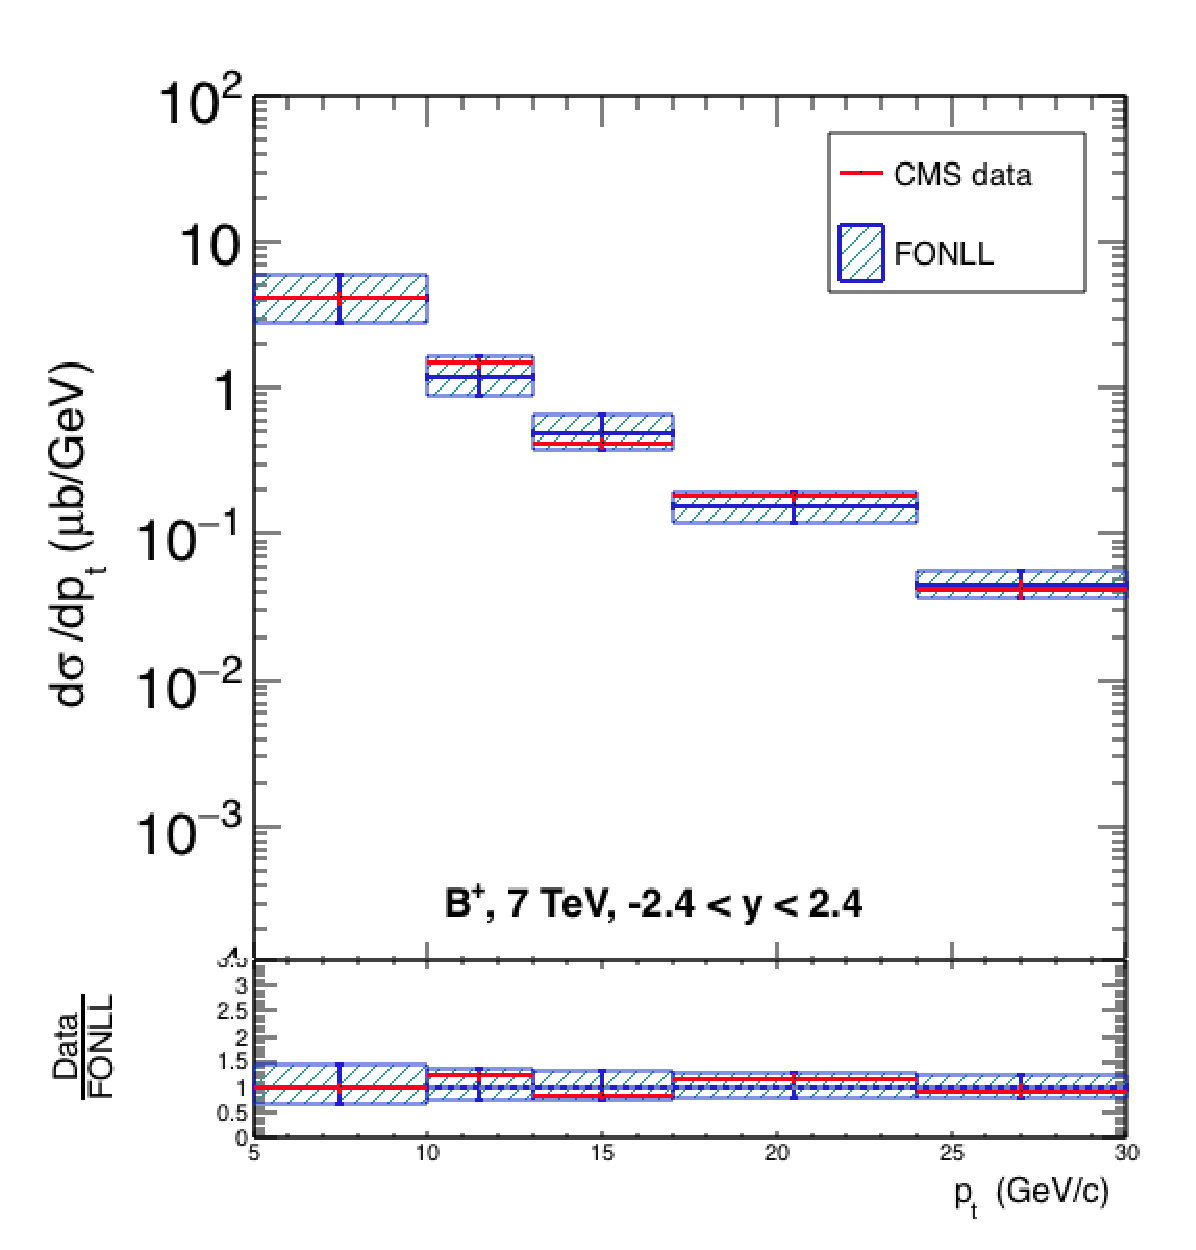
\includegraphics[width=.45\textwidth]{FigCap4/Bplus_7TeV_y_24_24.eps}
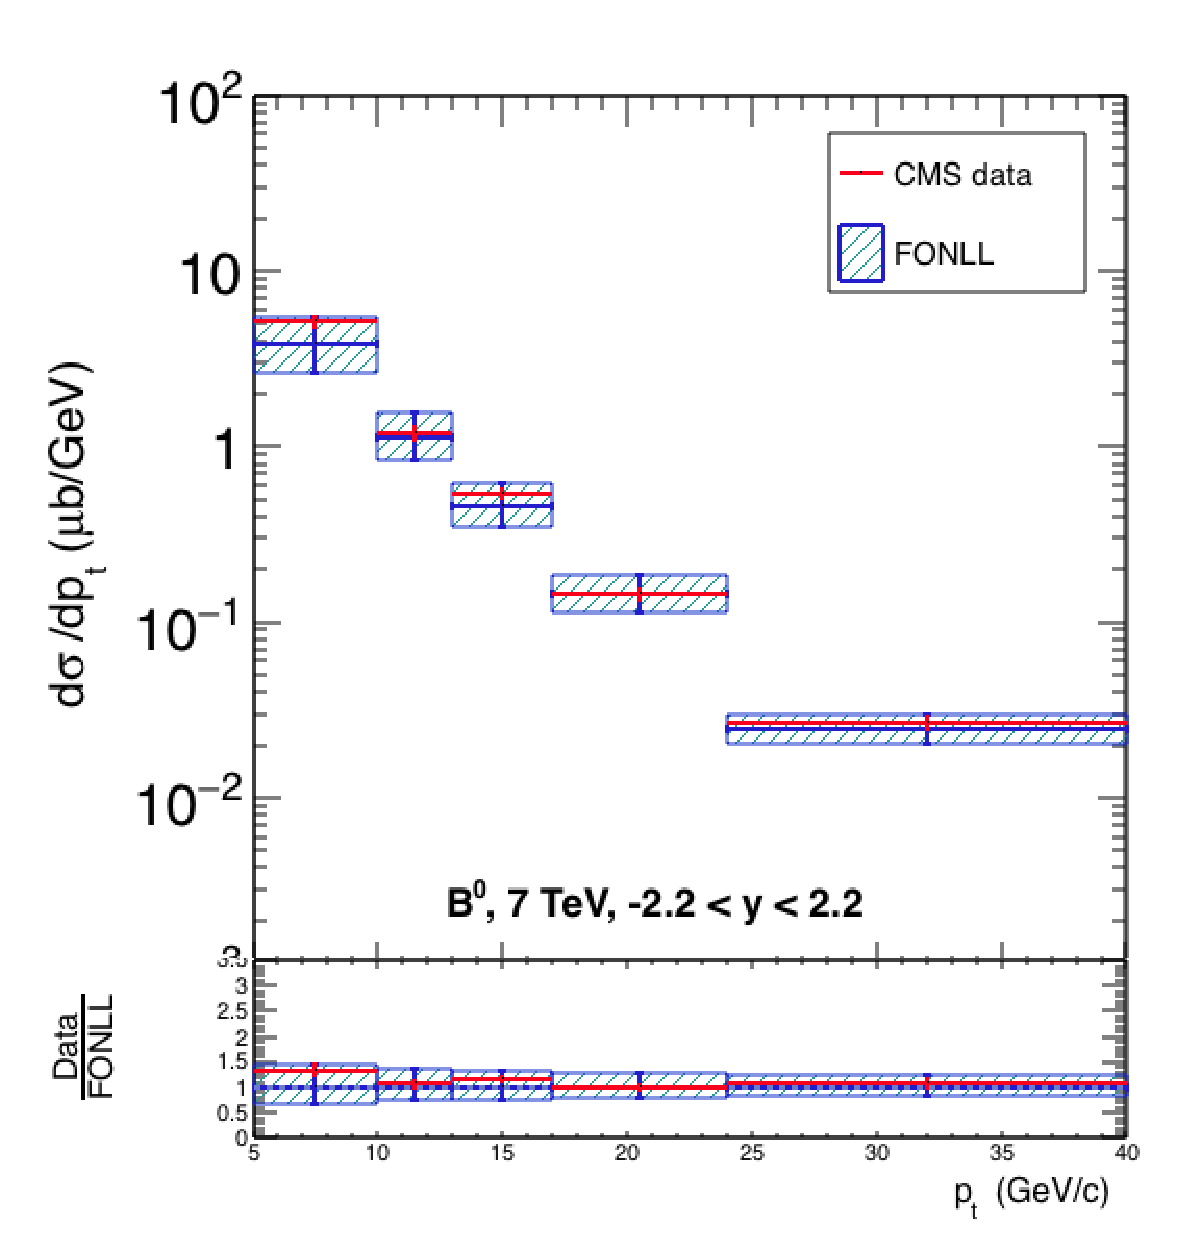
\includegraphics[width=.45\textwidth]{FigCap4/Bzero_7TeV_y_22_22.eps}
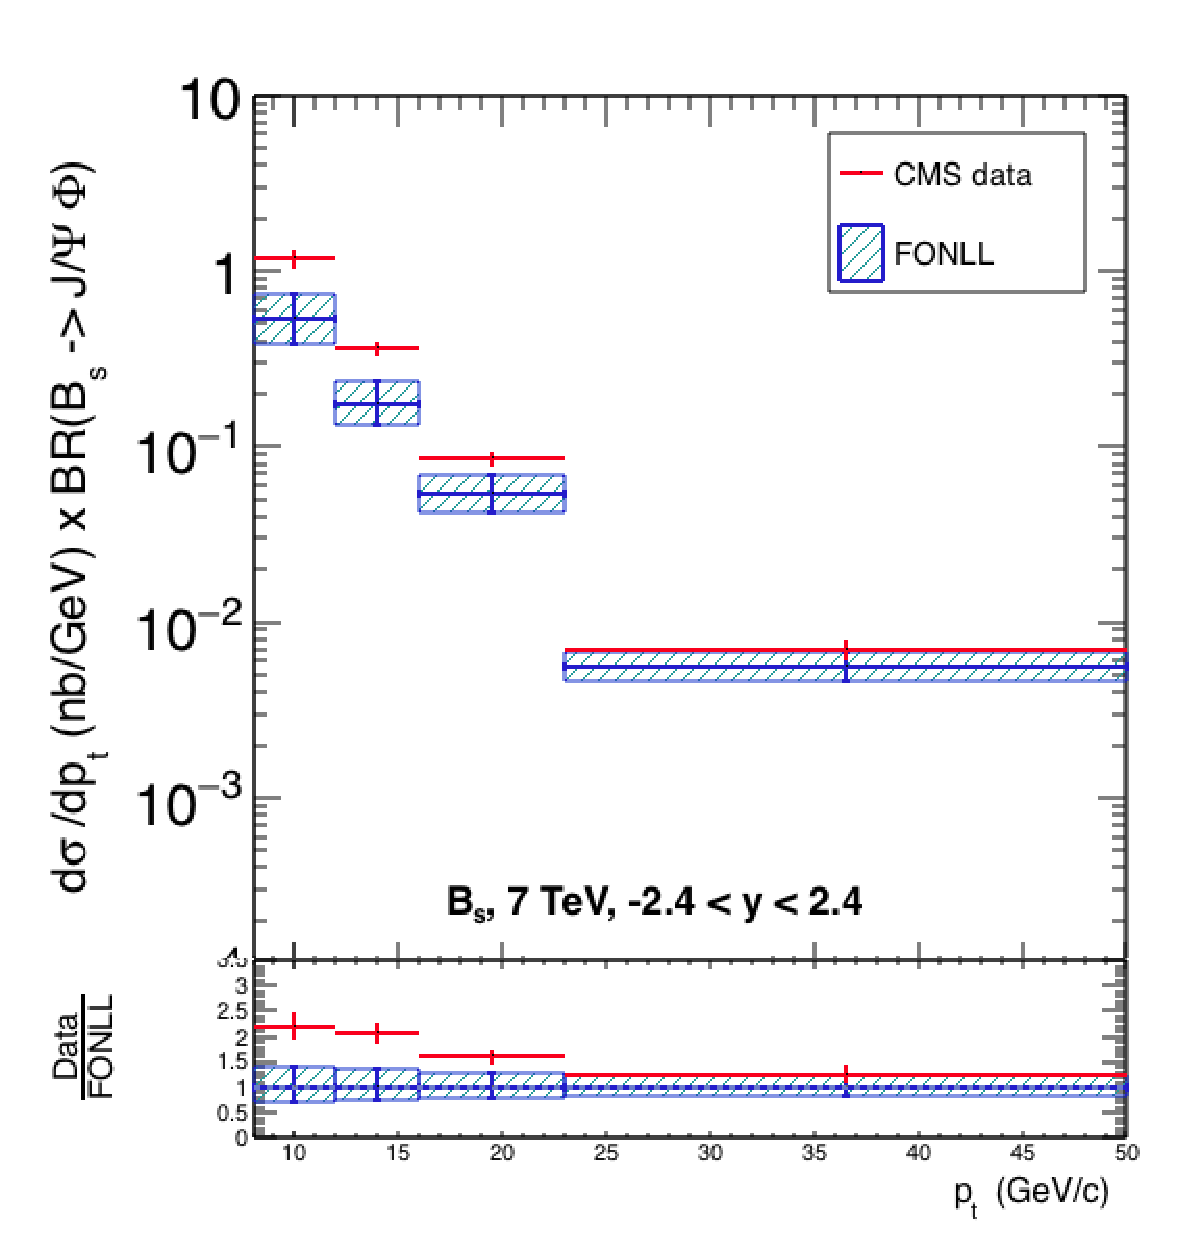
\includegraphics[width=.45\textwidth]{FigCap4/Bs_7TeV_y_24_24.eps}
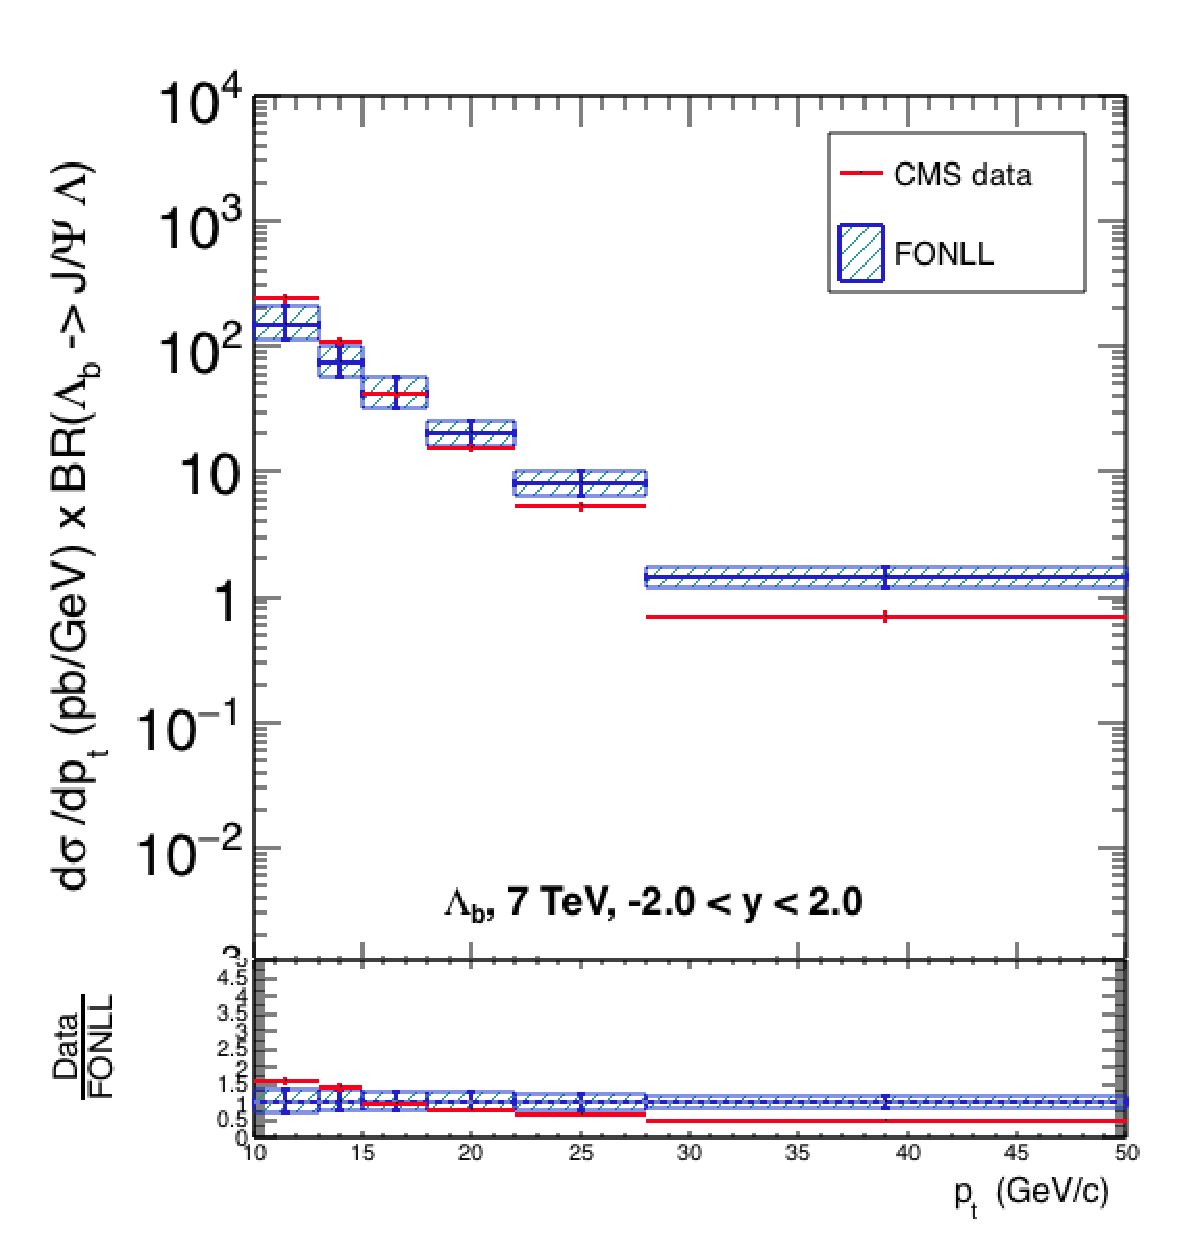
\includegraphics[width=.45\textwidth]{FigCap4/Lambdab_7TeV_y_20_20.eps}
\caption{B$^{+}$-, B$^{0}$-, B$_{\rm s}$-meson and $\Lambda_{\rm b}$-baryon differential cross-sections (red points) as a function of $\pt$ measured by CMS in pp collisions at $\s =$ 7 TeV at mid-rapidity~\cite{Khachatryan:2011mk,Chatrchyan:2011pw,Chatrchyan:2011vh,Chatrchyan:2012xg} compared to FONLL predictions~\cite{Cacciari:1998it, Cacciari:2001td} at the same energy (blue boxes). }
\label{fig:Bmesons}
\end{center}
\end{figure}

\begin{figure}[!htbp]
\begin{center}
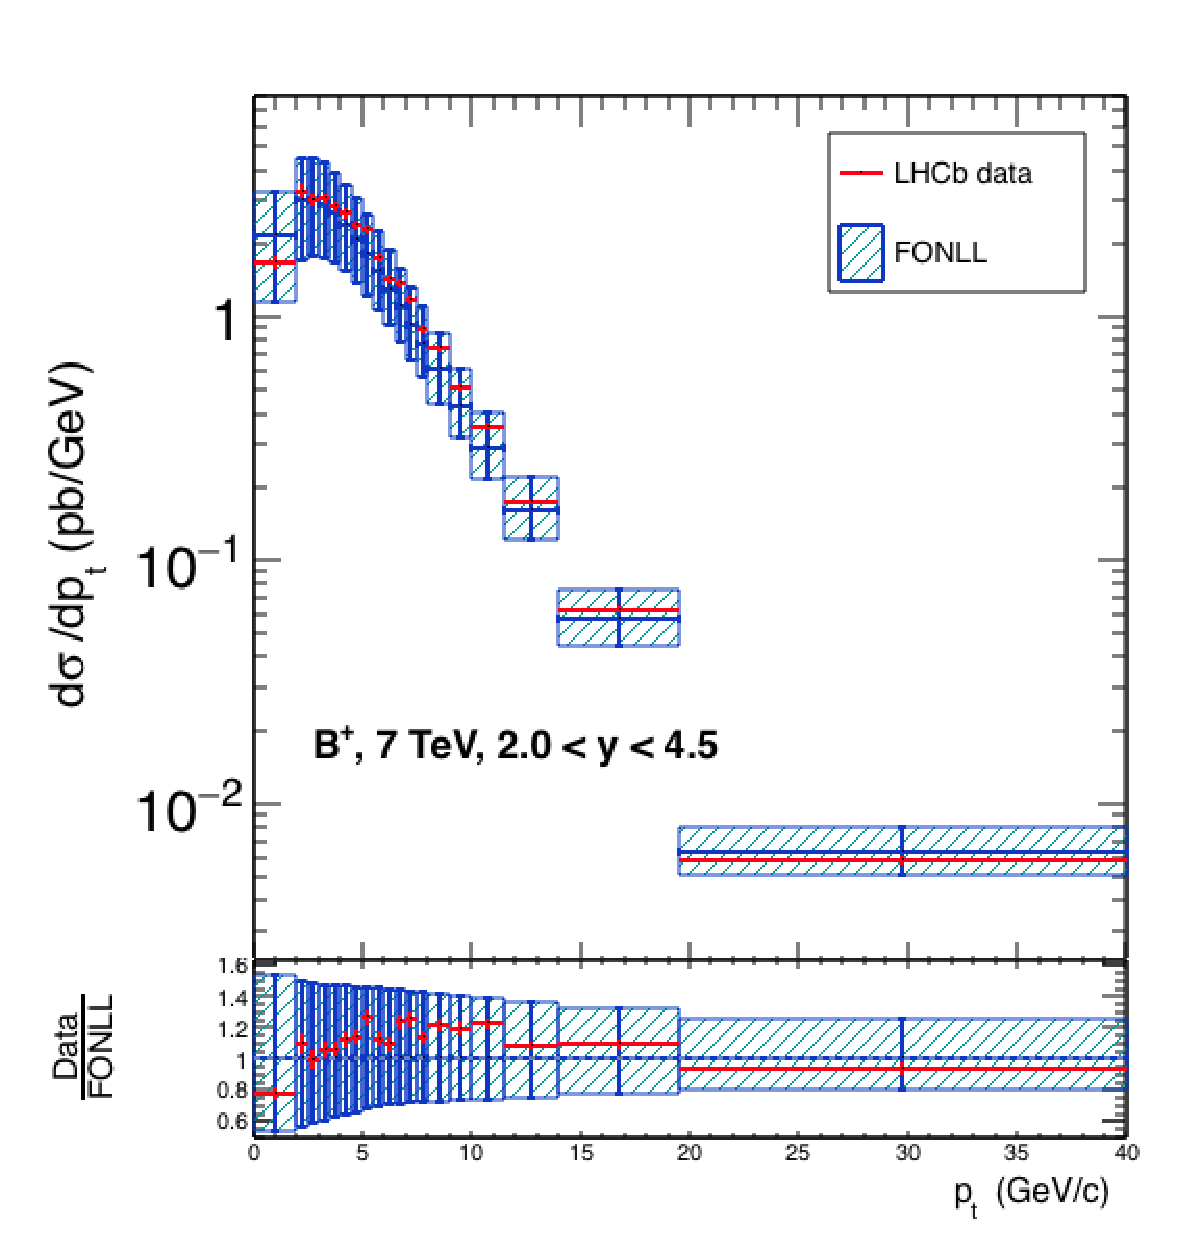
\includegraphics[width=.45\textwidth]{FigCap4/Bplus_7TeV_y_20_45_FF35.eps}
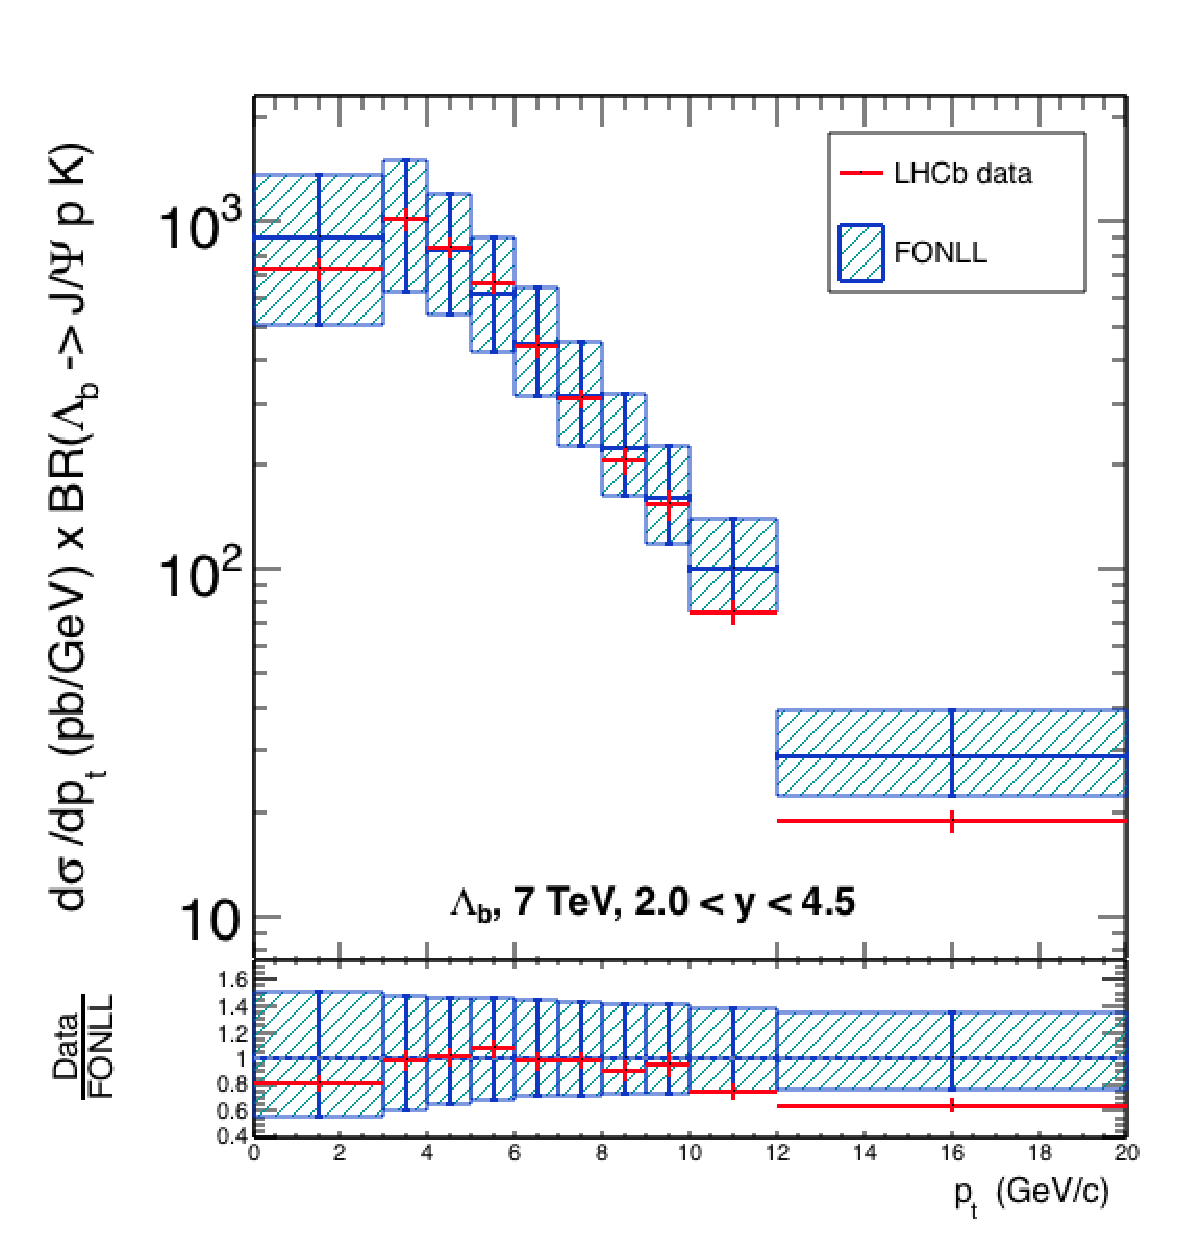
\includegraphics[width=.45\textwidth]{FigCap4/Lambdab_7TeV_y_20_45_FF21_BR6.eps}
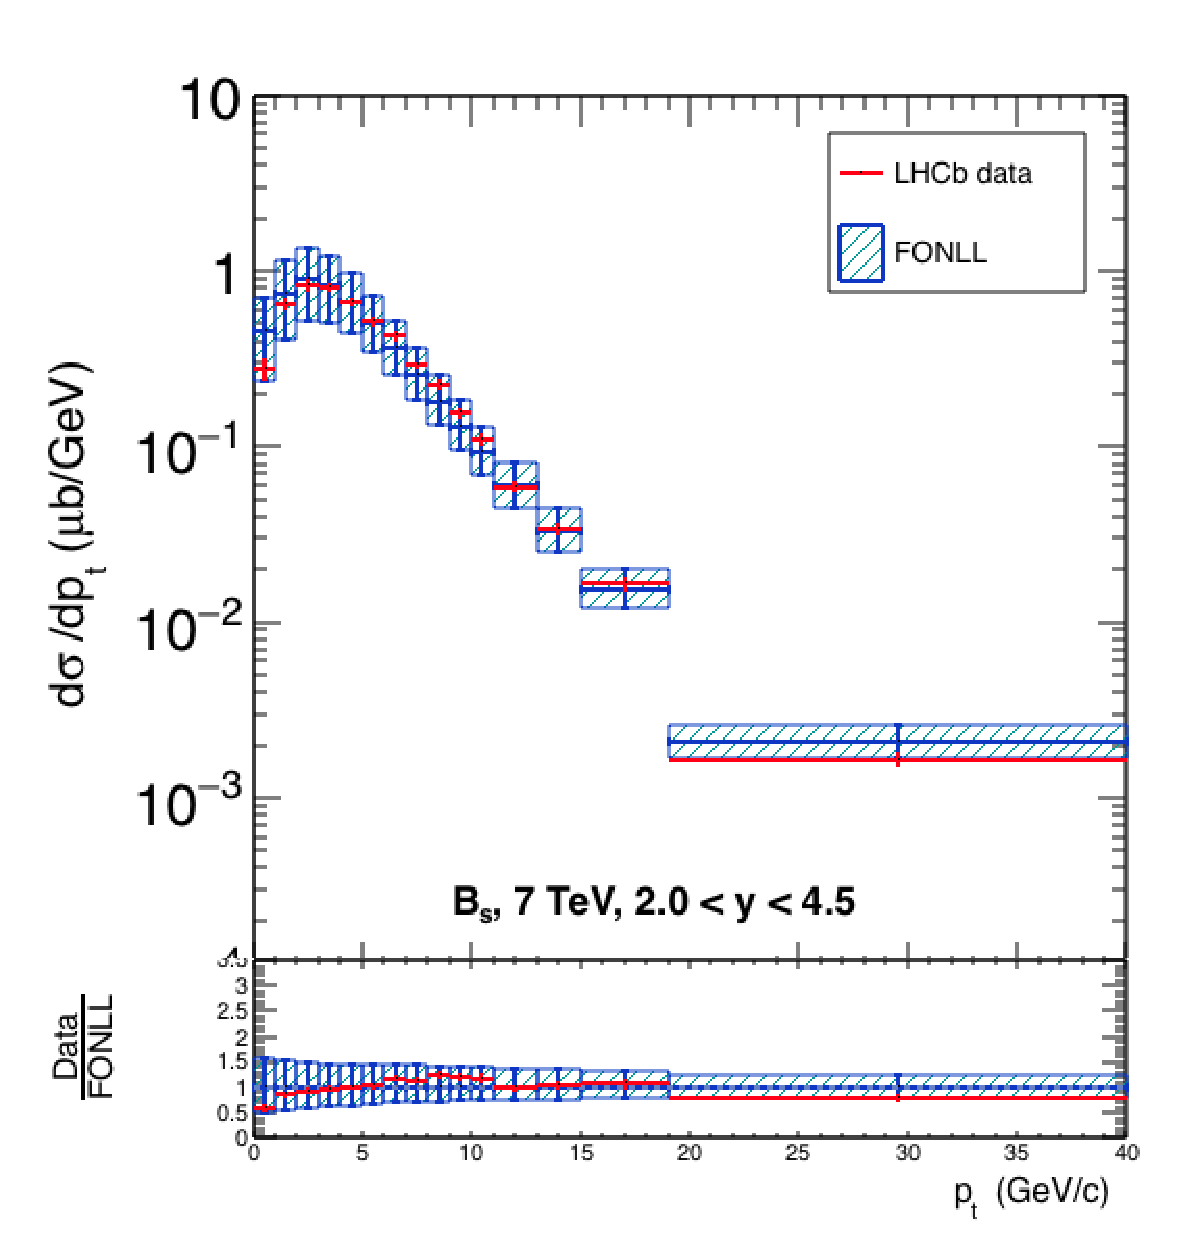
\includegraphics[width=.45\textwidth]{FigCap4/Bs_7TeV_y_20_45.eps}
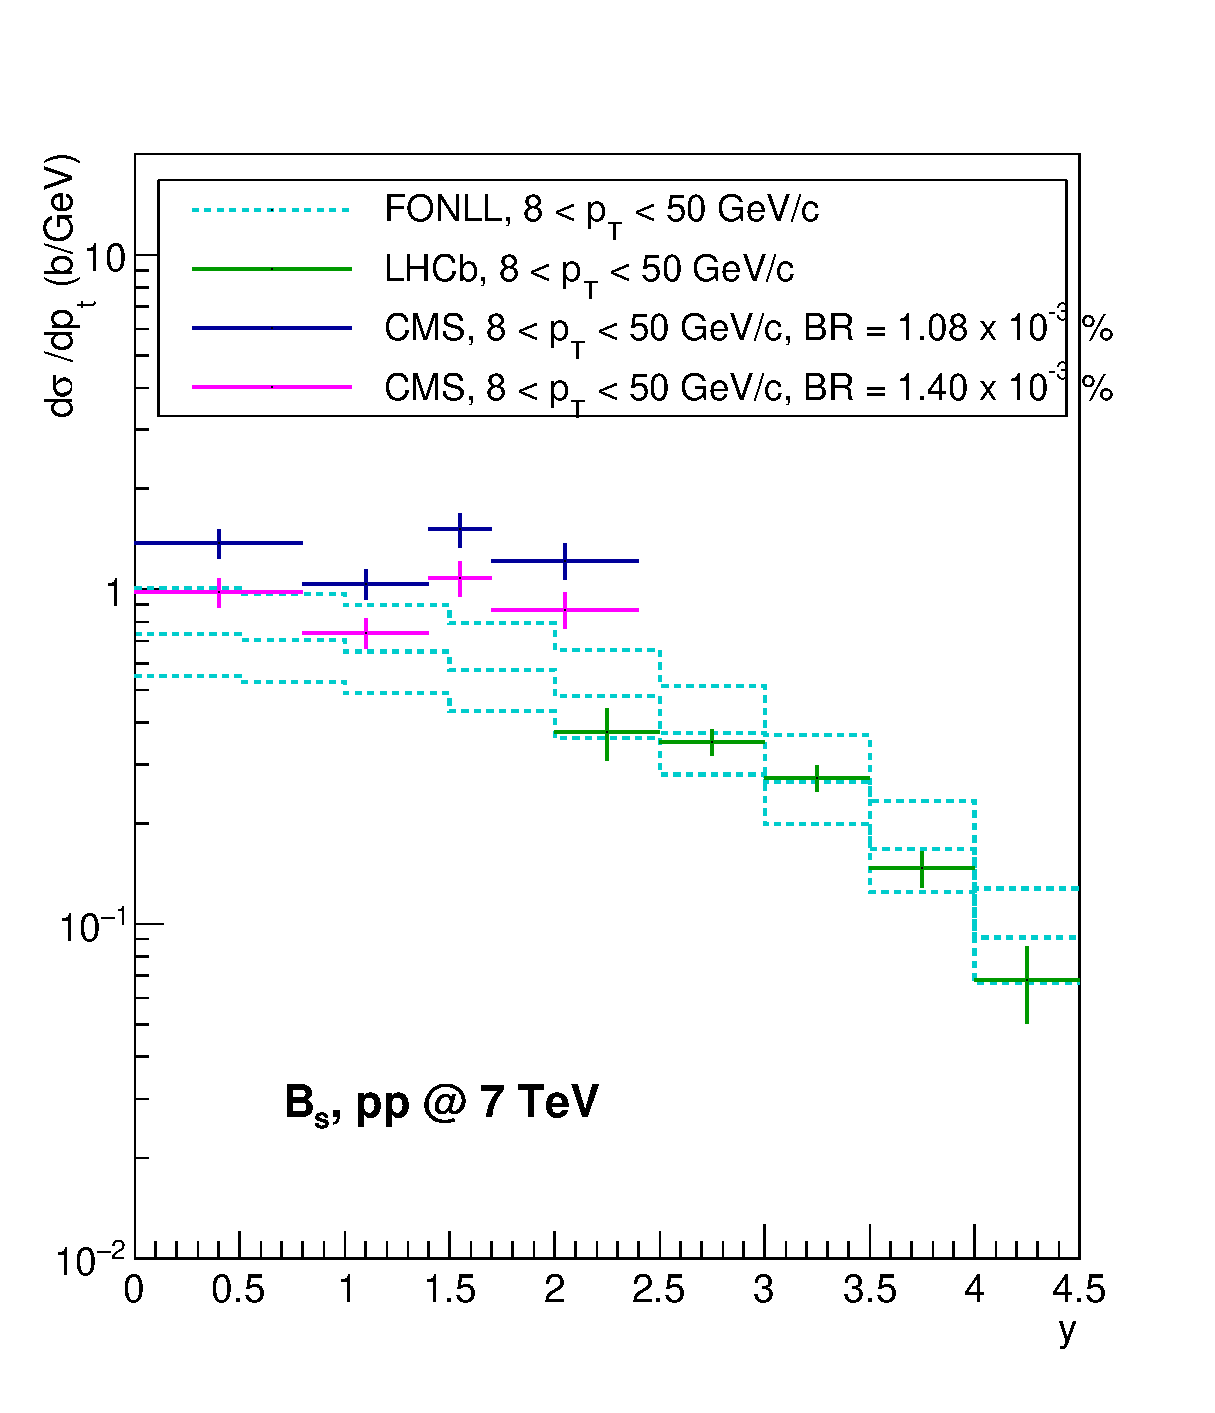
\includegraphics[width=.4\textwidth]{FigCap4/FONLL_CMSvsLHCb_3.eps}
\caption{B$^{+}$, $\Lambda_{\rm b}$ and B$^0_{\rm s}$ differential cross-sections (red points) measured by LHCb in pp collisions at $\s =$ 7 TeV at \mbox{2 $< y_{cm} <$ 4.5} compared to FONLL predictions at the same energy (blue boxes)~\cite{Aaij:2013noa,Aaij:2015fea}.
In the bottom right panel, B$^0_{\rm s}$-meson differential cross-section as a function of $y$ from LHCb is compared to same measurements from CMS at mid-rapidity (8 $< p_{\rm T} <$ 50 GeV/$c$) and to FONLL predictions~\cite{Cacciari:1998it, Cacciari:2001td} in the full rapidity range. }
\label{fig:LHCbBmesons}
\end{center}
\end{figure}


\begin{figure}[!htbp]
\begin{center}
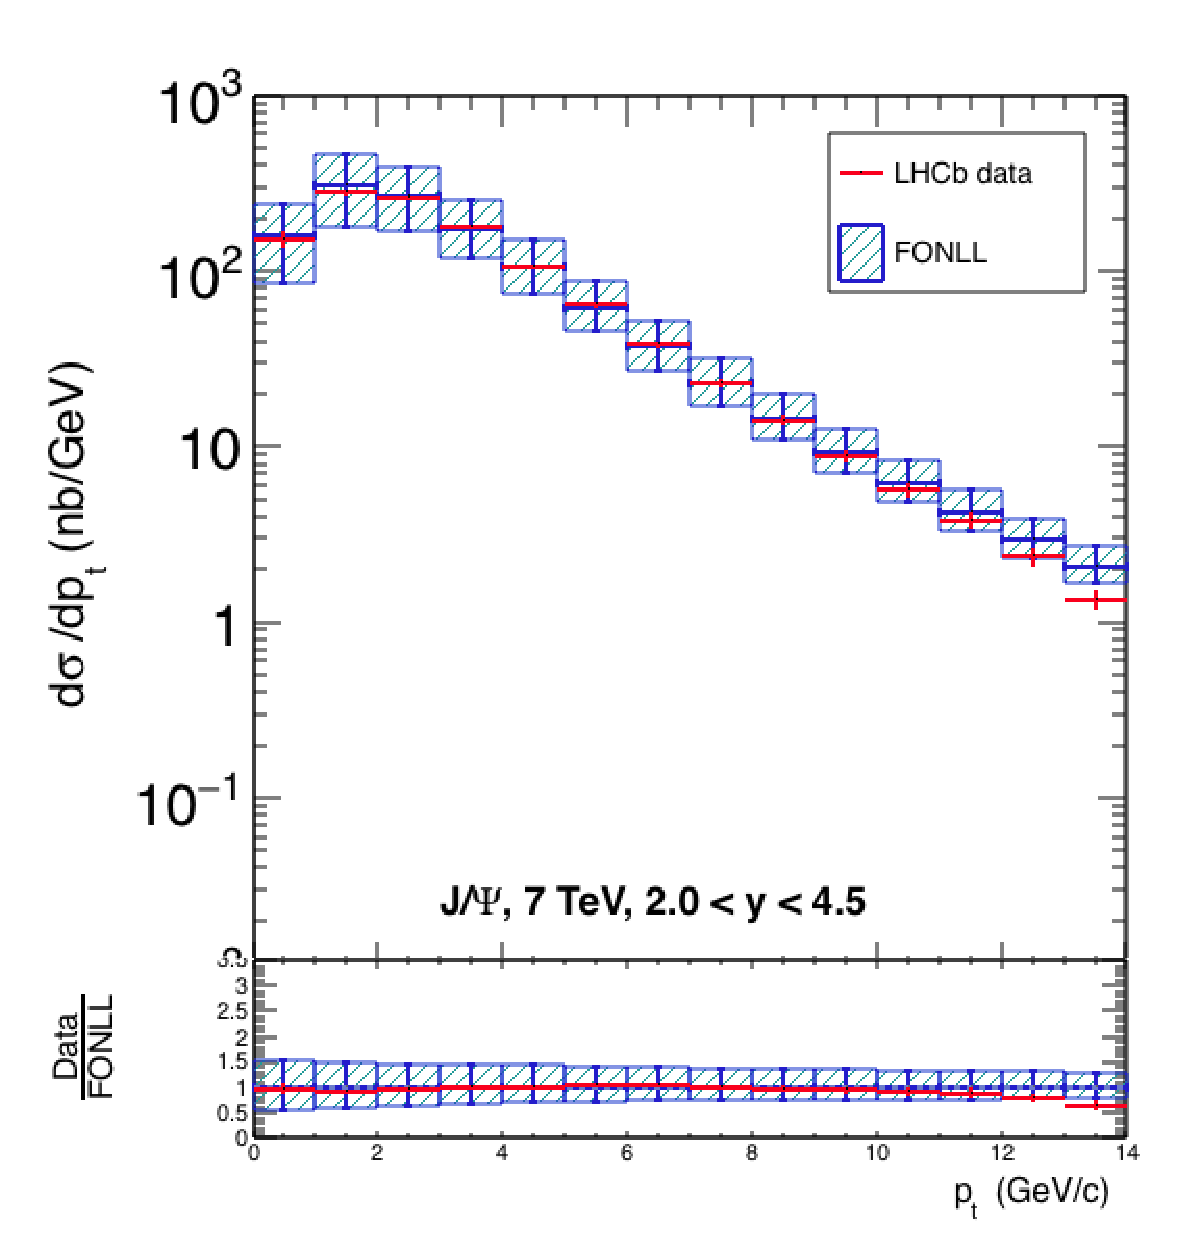
\includegraphics[width=.45\textwidth]{FigCap4/Jpsi_7TeV_y_20_45.eps}
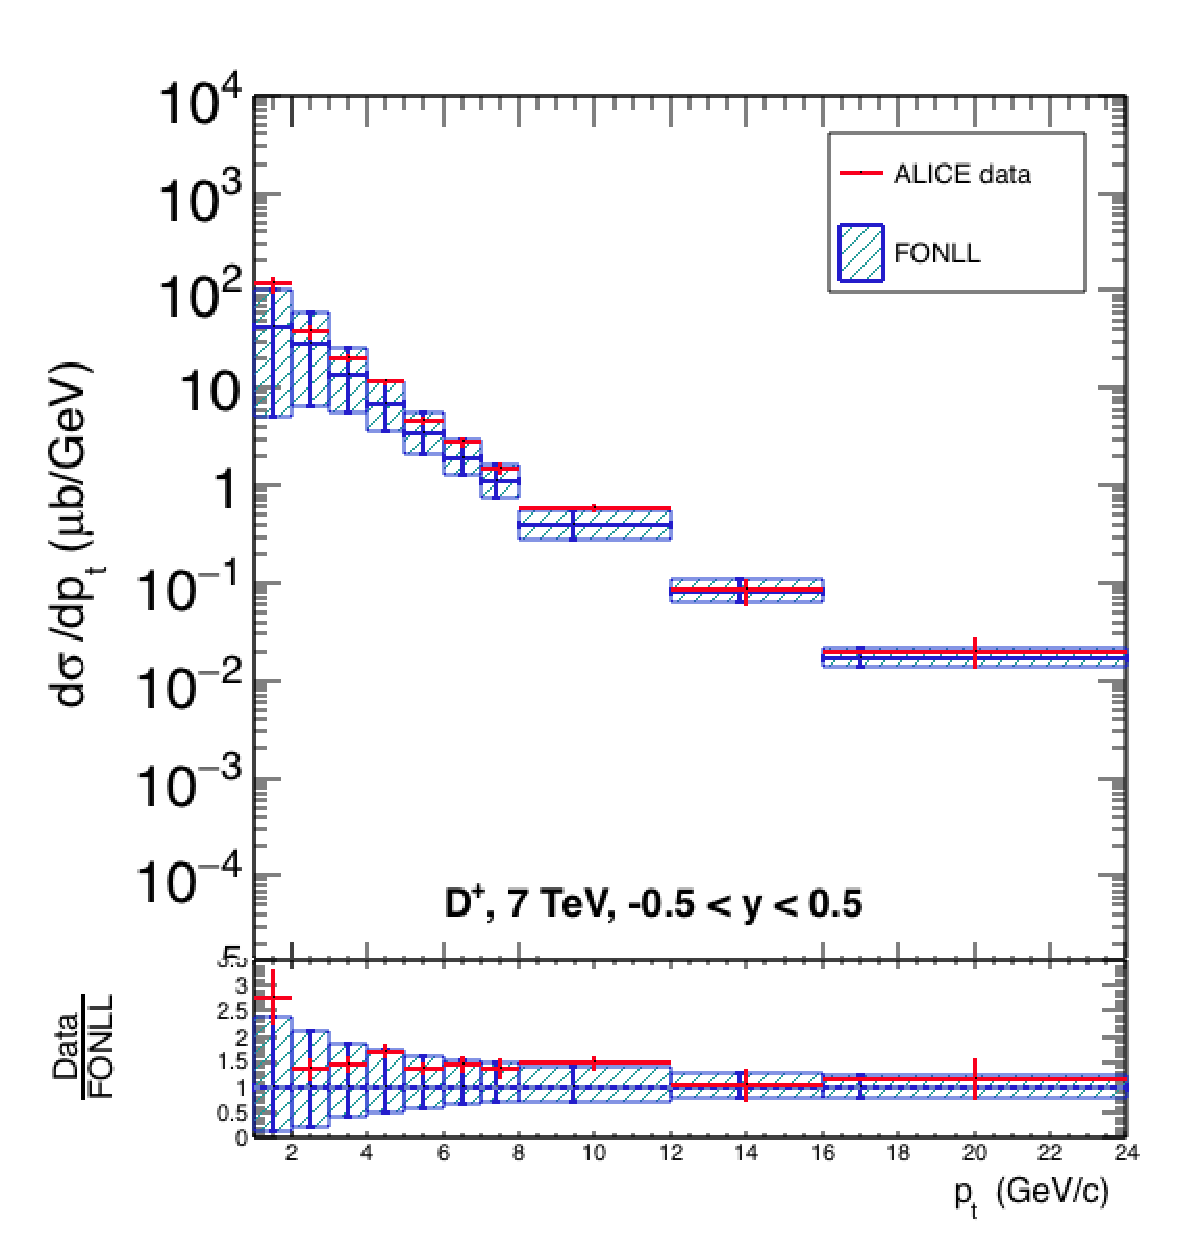
\includegraphics[width=.45\textwidth]{FigCap4/Dplus_7TeV_y_05_05.eps}
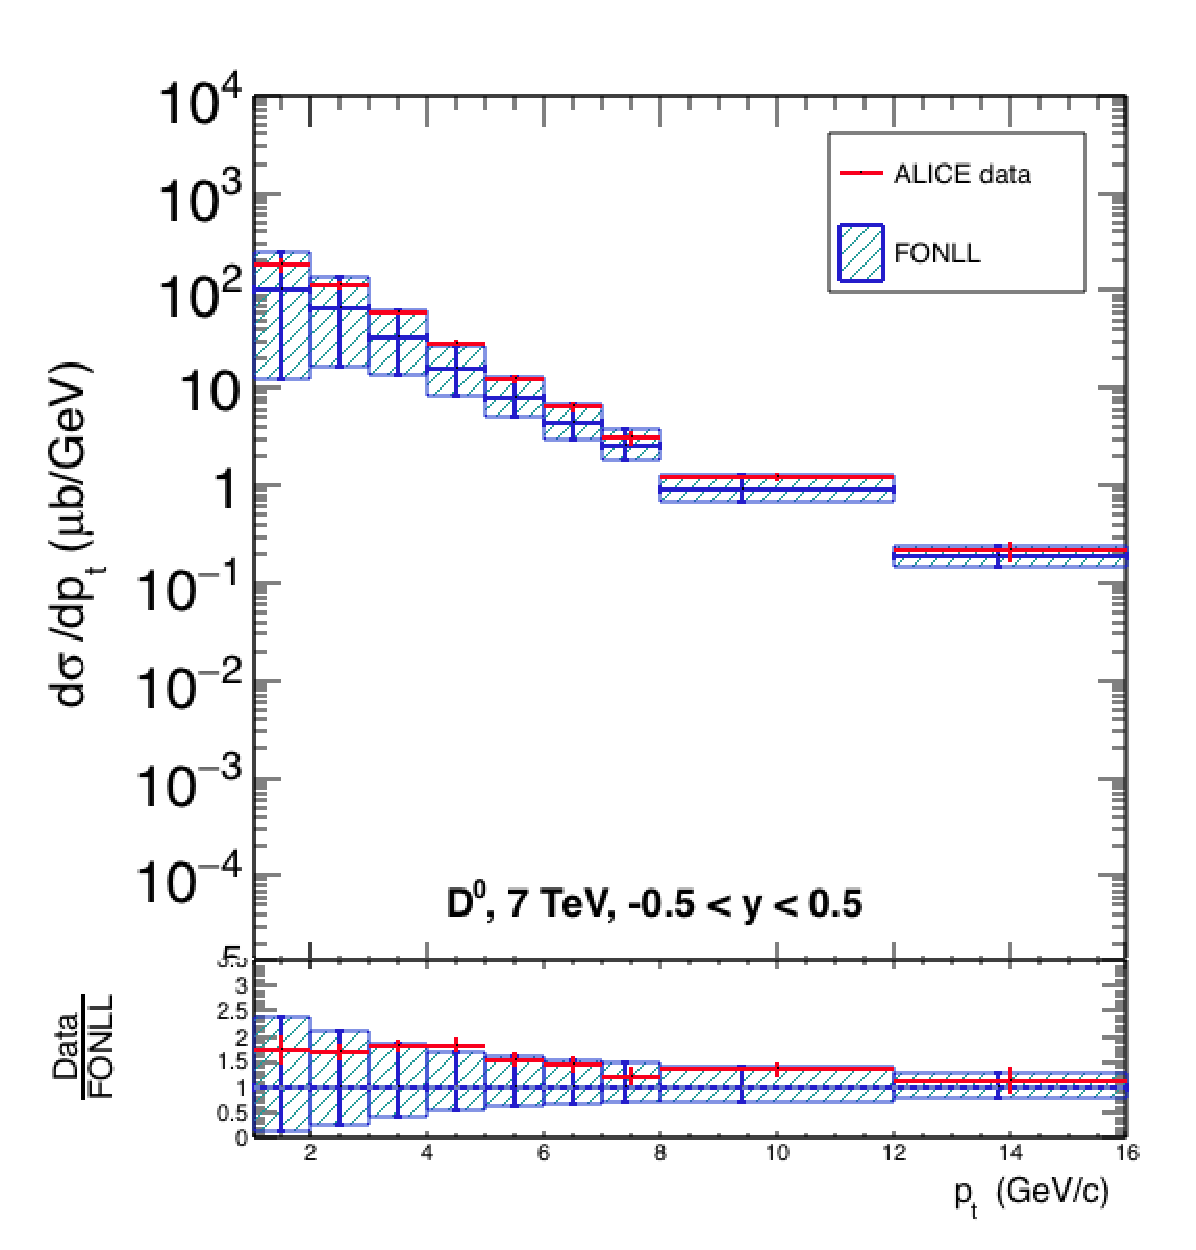
\includegraphics[width=.45\textwidth]{FigCap4/Dzero_7TeV_y_05_05.eps}
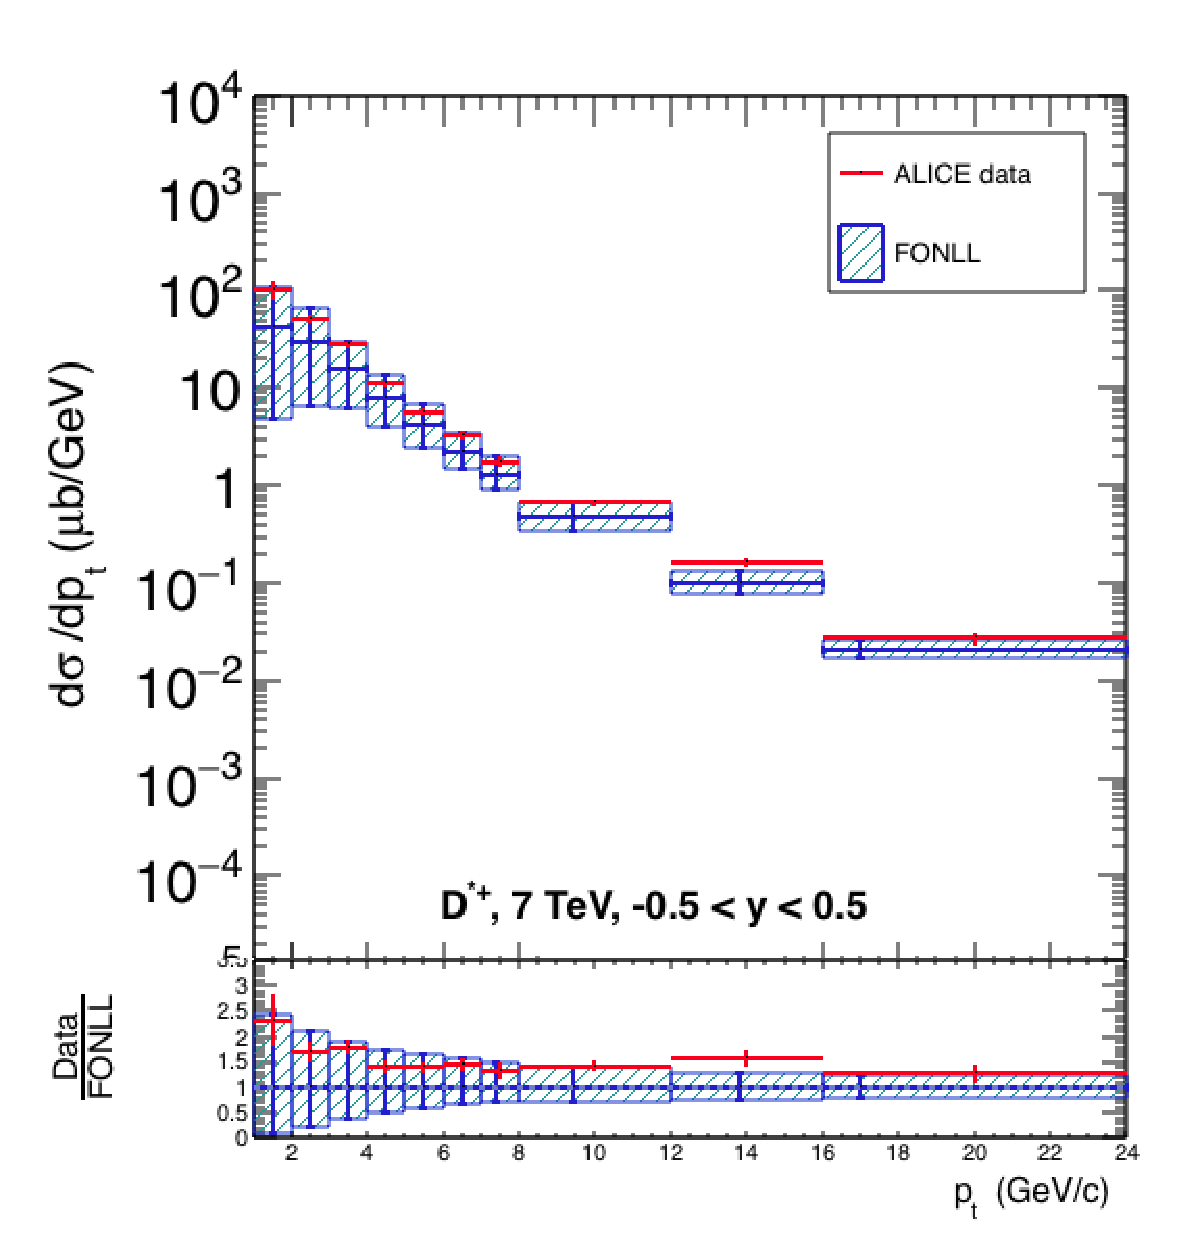
\includegraphics[width=.45\textwidth]{FigCap4/Dstar_7TeV_y_05_05.eps}
\caption{J/$\psi$- (from LHCb, \mbox{2 $< y_{cm} <$ 4.5}~\cite{Aaij:2011jh}), D$^{+}$-, D$^{0}$- and D$^+_{\rm s}$-meson (from ALICE, mid-rapidity~\cite{ALICE:2011aa}) differential cross-sections (red points) as a function of $\pt$ in pp collisions at $\s = $ 7 TeV compared to FONLL predictions~\cite{Cacciari:1998it, Cacciari:2001td} at the same energy (blue boxes). }
\label{fig:Dmesons}
\end{center}
\end{figure}
